\documentclass[11pt]{article}

\usepackage[margin=1in]{geometry}
\usepackage{amsmath}
\usepackage{amssymb}
\usepackage{amsfonts}
\usepackage{amsthm}
\usepackage{enumitem}
\usepackage{tikz}

\newtheoremstyle{solstyle}{6pt}{6pt}{}{}{\bfseries}{.}{ }{}
\theoremstyle{solstyle}
\newtheorem*{solution}{Solution}

\tikzset{v/.style={circle,fill=black,inner sep=1.5pt}}

\newcommand{\glabel}[1]{\begin{center}\textbf{[Graph #1]}\end{center}}

\setlength{\parindent}{0pt}
\setlength{\parskip}{6pt}

\begin{document}

\noindent\textbf{"Group Name"}\hfill\textbf{Jul 22, 2026}

\noindent\textbf{Clarifier:} Changhwan\\
\textbf{Manager:} Henry\\
\textbf{Reporter:} Benjamin\\
\textbf{Skeptic:} Sharan

\textbf{Report: Today's tasks went well. We have identified the relation between many problems and Harris graphs. The other questions were solved relatively quickly, though number 5 caught us for a while. } 
% And yes, I was fired, but that was because i was translating the ENTIRE THING to tek......

\begin{center}\rule{0.6\textwidth}{0.4pt}\end{center}

\textbf{SOLUTIONS \& PROOFS:} \\
Without Loss of Generality is abbreviated as WLoG within this document. 

\begin{enumerate}[leftmargin=*]

\item Prove the following is a sufficient condition for a graph to be Hamiltonian: a graph is Hamiltonian if $n > 2$ and the minimum degree of every vertex is at least $n/2$.

\begin{proof}
Let $u,v$ be any two nonadjacent vertices. Then $\deg(u)+\deg(v) \geq n/2 + n/2 = n$, so $G$ satisfies Ore's condition, and is therefore Hamiltonian.
\end{proof}

\begin{proof}
Non-Ore utilizing proof. 
Let $G$ be a graph on $n \geq 3$ vertices with $deg(G) \geq n/2$.

\textbf{$G$ is connected.} If not, take a smallest component $H$. Every vertex of $H$ has all its neighbors inside $H$, so $|V(H)| \geq deg(G) + 1 > n/2$. A second component is at least as large, giving more than $n$ vertices total, a contradiction.

\textbf{A longest path spans a cycle.} Let $P = v_0 v_1 \cdots v_k$ be a longest path in $G$. By maximality every neighbor of $v_0$ and every neighbor of $v_k$ lies on $P$; otherwise $P$ extends. Define
$$A = \{\, i : v_0 v_i \in E \,\}, \qquad B = \{\, i : v_{i-1} v_k \in E \,\},$$
both subsets of $\{1, \dots, k\}$. Then $|A| = deg(v_0) \geq n/2$ and $|B| = deg(v_k) \geq n/2$, so $|A| + |B| \geq n > k$. Since $\{1,\dots,k\}$ has only $k$ elements, $A \cap B \neq \varnothing$. Pick $i \in A \cap B$, so $v_0 v_i \in E$ and $v_{i-1} v_k \in E$. Then
$$C : v_0 \, v_1 \cdots v_{i-1} \, v_k \, v_{k-1} \cdots v_i \, v_0$$
is a cycle containing every vertex of $P$.

\textbf{$C$ is Hamiltonian.} Suppose some vertex $u$ lies outside $C$. As $G$ is connected, $u$ has a neighbor $v_j \in C$. Cutting $C$ at $v_j$ gives a path through all $k+1$ vertices of $C$ starting at $v_j$, and prepending $u$ yields a path on $k+2$ vertices, longer than $P$, a contradiction. Hence $C$ contains all $n$ vertices and is a Hamiltonian cycle.
\end{proof}




\item Prove or disprove : The following graph is Hamiltonian.
\begin{center}
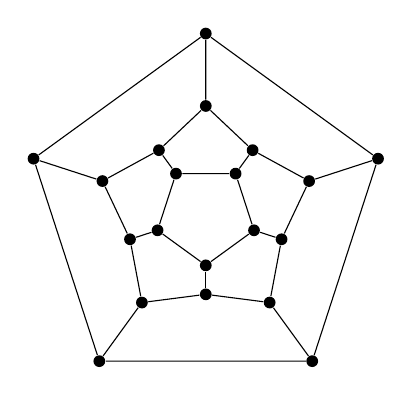
\begin{tikzpicture}[scale=0.92]
\node[v] (A1) at (90:2.5){};
\node[v] (A2) at (18:2.5){};
\node[v] (A3) at (-54:2.5){};
\node[v] (A4) at (-126:2.5){};
\node[v] (A5) at (162:2.5){};
\node[v] (A6) at (90:1.5){};
\node[v] (A7) at (18:1.5){};
\node[v] (A8) at (-54:1.5){};
\node[v] (A9) at (-126:1.5){};
\node[v] (A10) at (162:1.5){};

\node[v] (A11) at (-90:1.1){};
\node[v] (A12) at (-18:1.1){};
\node[v] (A13) at (54:1.1){};
\node[v] (A14) at (126:1.1){};
\node[v] (A15) at (-162:1.1){};

\node[v] (A16) at (-90:0.7){};
\node[v] (A17) at (-18:0.7){};
\node[v] (A18) at (54:0.7){};
\node[v] (A19) at (126:0.7){};
\node[v] (A20) at (-162:0.7){};



\draw (A1)--(A2)--(A3)--(A4)--(A5)--(A1);
\draw (A1)--(A6) (A2)--(A7) (A3)--(A8) (A4)--(A9) (A5)--(A10);
\draw (A6)--(A13)--(A7)--(A12)--(A8)--(A11)--(A9)--(A15)--(A10)--(A14)--(A6);
\draw (A11)--(A16);
\draw (A12)--(A17);
\draw (A13)--(A18);
\draw (A14)--(A19);
\draw (A15)--(A20);
\draw (A16)--(A17)--(A18)--(A19)--(A20)--(A16);

\end{tikzpicture}
\end{center}
\glabel{I}
\begin{solution}
Proved. 
\end{solution}
\begin{proof}
We show that this graph is Hamiltonian, as shown in the following path:
\newline
$$18\rightarrow 19 \rightarrow 20 \rightarrow 16 \rightarrow 17 \rightarrow 7 \rightarrow 6 \rightarrow 15 \rightarrow 14 \rightarrow 13 \rightarrow $$

$$12 \rightarrow 11 \rightarrow 10 \rightarrow 3 \rightarrow 2 \rightarrow 1 \rightarrow 5 \rightarrow 8 \rightarrow 9 \rightarrow 18$$
Thus, since there exists a path across every vertex, the graph is Hamiltonian. 
\end{proof}

\item Prove or disprove
\begin{enumerate}[label=(\alph*),leftmargin=*]

\item All Eulerian graphs are Hamiltonian.
\begin{solution}
    Disproved. 
\end{solution}
\begin{proof}
Counterexample. 
\begin{center}
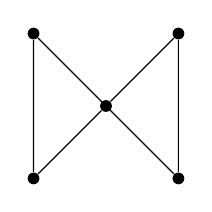
\begin{tikzpicture}[scale=0.92]
\node[v] (A1) at (-1, 1){};
\node[v] (A2) at (-1, -1){};
\node[v] (A3) at (0, 0){};
\node[v] (A4) at (1, 1){};
\node[v] (A5) at (1, -1){};
\draw (A1)--(A2)--(A3)--(A4)--(A5)--(A1);

\end{tikzpicture}
\end{center}
\glabel{II}
\end{proof}
\item All Hamiltonian graphs are Eulerian.
\begin{solution}
    Disproved. 
\end{solution}
\begin{proof}
Counterexample. 
\begin{center}
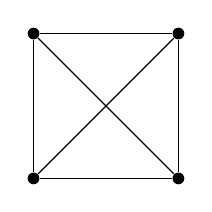
\begin{tikzpicture}[scale=0.92]
\node[v] (A1) at (0, 0){};
\node[v] (A2) at (0, 2){};
\node[v] (A3) at (2, 2){};
\node[v] (A4) at (2, 0){};
\draw (A1)--(A2)--(A3)--(A4)--(A1);
\draw (A1)--(A3) (A2)--(A4);

\end{tikzpicture}
\end{center}
\glabel{III}
\end{proof}
\item All 2-connected, Eulerian graphs are Hamiltonian.
\begin{solution}
    Disproved. 
\end{solution}
\begin{proof}
Let us tighten the given constraints. 2-connectedness is included in the definition of toughness, in the special case of $n_r=2$, where $n_r$ shows the number of removed vertices. Therefore, if the claim is disproved for a tough graph, it will be disproved for a 2-connected graph. 

However, a 2-connected, Eulerian graph is known not to result in a Hamiltonian graph via the Harris graph disproval. Therefore, any Harris graph is a counterexample to this claim. 
\end{proof}

\end{enumerate}
\item Prove that having no odd cycles is a necessary condition for a graph to be bipartite.
\begin{proof}
Suppose not. Our claim is that there is a bipartite graph with an odd cycle. Let us call that cycle length $N$. Let us select an arbitrary point inside the cycle as $v_1$. Since this graph is bipartite, we should be able to label all points inside two disjoint sets, $A$ and $B$. WLoG $v_1 \in A$. since the two sets are disjoint and each set doesn't have edges within itself, we can see that $v_{2k+1} \in A$ and $v_{2k} \in B$ for some $k \in \mathbb{Z}$ and $2k+1 \leq N$. However, since $v_1$ and $v_{N}$ are in the same set $A$, we cannot draw the edge $v_1 v_{N}$ and therefore cannot complete the cycle. 

We have reached a contradiction. Therefore, for a graph to be bipartite, it must have no odd cycles. 
\end{proof}

\item Prove that having no odd cycles is also a sufficient condition for a graph to be bipartite. 

\begin{proof}
    We begin by defining a tree as a connecting graph containing no cycle, and a spanning tree as any maximal (connected) subgraph containing no cycles and every vertex. We note that having no odd cycles leaves the graph with subgraphs that either contain even cycles or trees. We also note that trees (and consequently, spanning trees) are bipartite as each child node can be colored the opposite of its parent node, starting with an arbitrary choice at the root $R$. Now, we take the graph $G$ and take a subgraph $S_G$ such that it is a spanning tree. As shown before, $S_G$ is bipartite.  
    
    It remains to show that any edge we re-add to $S_G$ to obtain $G$ again does not connect any two vertices of the same color. We prove this by contradiction. Suppose there did exist two vertices $x$ and $y$ of the same color, such that there were an edge between them. Then the distance from $x$ to $y$ would become $1,$ and as $G$ contains no odd cycles, the path $x\rightarrow y$ through $R$ must be of odd length. However, this path is equivalent to the sum of the distances of $x\rightarrow R$ and $y\rightarrow R.$ As the sum is odd, one of the two path lengths must be odd, and the other even. As the colors alternate between parent and child, the color of $x$ then cannot equal the color of $y,$ forcing a contradiction.
\end{proof}

\item Consider this sufficiency condition : A graph is Hamiltonian if it is 2 connected and does not contain $K_{1,3}$ nor $K_{1, 3} + x$ as an induced subgraph. 

\begin{center}
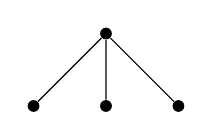
\begin{tikzpicture}[scale=0.92]
\node[v] (A1) at (0, 0){};
\node[v] (A2) at (-1, -1){};
\node[v] (A3) at (0, -1){};
\node[v] (A4) at (1, -1){};
\draw (A1)--(A2) (A1)--(A3) (A1)--(A4);
\end{tikzpicture}
\qquad
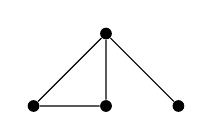
\begin{tikzpicture}[scale=0.92]
\node[v] (A1) at (0, 0){};
\node[v] (A2) at (-1, -1){};
\node[v] (A3) at (0, -1){};
\node[v] (A4) at (1, -1){};
\draw (A1)--(A2) (A1)--(A3) (A1)--(A4) (A2)--(A3);
\end{tikzpicture}
\end{center}
\glabel{IV}

Prove that this is not a necessary condition. 
\begin{proof}
Counterexample. 
\begin{center}
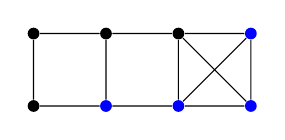
\begin{tikzpicture}[scale=0.92]
\node[v] (A1) at (0, 0){};
\node[v,fill=blue] (A2) at (1, 0){};
\node[v,fill=blue] (A3) at (2, 0){};
\node[v,fill=blue] (A4) at (3, 0){};
\node[v] (A5) at (0, 1){};
\node[v] (A6) at (1, 1){};
\node[v] (A7) at (2, 1){};
\node[v,fill=blue] (A8) at (3, 1){};
\draw (A1)--(A2)--(A3)--(A4)--(A8)--(A7)--(A6)--(A5)--(A1) (A2)--(A6) (A3)--(A7) (A4)--(A7) (A3)--(A8);
\end{tikzpicture}
\end{center}
\glabel{V}
\end{proof}
\item Prove that 3-regular("cubic") + connected + no odd cycles is \textit{not} a sufficient condition for being Hamiltonian. 
\begin{proof}
Counterexample. Cubic, connected, and bipartite (left column with $w$ vs. right column with $u$), but deleting the two hubs $u,w$ leaves three components, so it is not tough and hence non-Hamiltonian.
\begin{center}
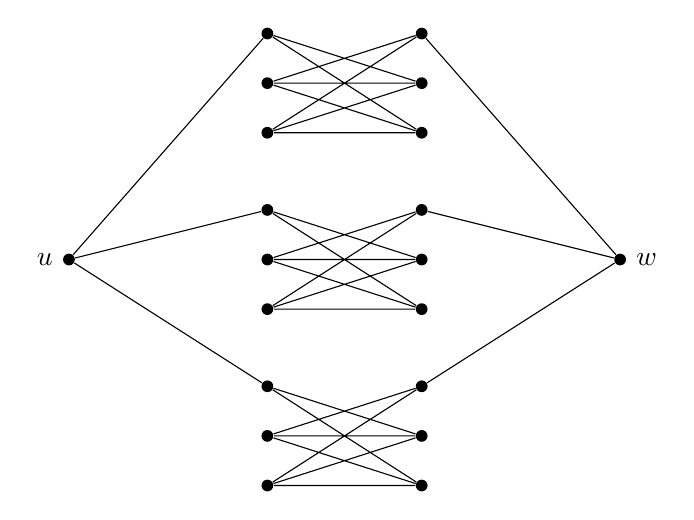
\begin{tikzpicture}[scale=0.7]
% hubs
\node[v,label=left:{$u$}]  (u) at (-5,0){};
\node[v,label=right:{$w$}] (w) at (5,0){};

% Lobe 1 (top)
\node[v] (p1) at (-1.4, 4.1){};
\node[v] (b1) at (-1.4, 3.2){};
\node[v] (e1) at (-1.4, 2.3){};
\node[v] (q1) at (1.4, 4.1){};
\node[v] (a1) at (1.4, 3.2){};
\node[v] (f1) at (1.4, 2.3){};

% Lobe 2 (middle)
\node[v] (p2) at (-1.4, 0.9){};
\node[v] (b2) at (-1.4, 0){};
\node[v] (e2) at (-1.4, -0.9){};
\node[v] (q2) at (1.4, 0.9){};
\node[v] (a2) at (1.4, 0){};
\node[v] (f2) at (1.4, -0.9){};

% Lobe 3 (bottom)
\node[v] (p3) at (-1.4, -2.3){};
\node[v] (b3) at (-1.4, -3.2){};
\node[v] (e3) at (-1.4, -4.1){};
\node[v] (q3) at (1.4, -2.3){};
\node[v] (a3) at (1.4, -3.2){};
\node[v] (f3) at (1.4, -4.1){};

% lobe edges (K_{3,3} minus one edge, each lobe)
\draw (p1)--(a1) (p1)--(f1) (b1)--(q1) (b1)--(a1) (b1)--(f1) (e1)--(q1) (e1)--(a1) (e1)--(f1);
\draw (p2)--(a2) (p2)--(f2) (b2)--(q2) (b2)--(a2) (b2)--(f2) (e2)--(q2) (e2)--(a2) (e2)--(f2);
\draw (p3)--(a3) (p3)--(f3) (b3)--(q3) (b3)--(a3) (b3)--(f3) (e3)--(q3) (e3)--(a3) (e3)--(f3);

% door edges to hubs
\draw (u)--(p1) (u)--(p2) (u)--(p3);
\draw (w)--(q1) (w)--(q2) (w)--(q3);
\end{tikzpicture}
\end{center}
\glabel{VI}
\end{proof}
\item Convert the "Patrolling the Palace" problem into a graph theory problem and solve it. 
\begin{solution}
    Once converted, we cannot find the Hamiltonian cycle on this graph. 
\end{solution}
\begin{proof}
Convert each room in the museum into a vertex, and neighboring connections to the rooms be edges. we end up with the following graph : 
\begin{center}
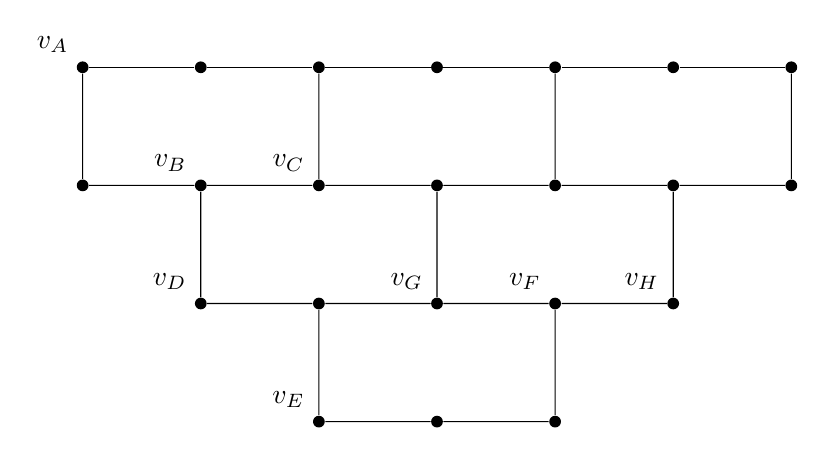
\begin{tikzpicture}[scale=1.5]
\node[v, label=above left:{$v_A$}] (A11) at (0, 0){};
\node[v] (A12) at (1, 0){};
\node[v] (A13) at (2, 0){};
\node[v] (A14) at (3, 0){};
\node[v] (A15) at (4, 0){};
\node[v] (A16) at (5, 0){};
\node[v] (A17) at (6, 0){};
\draw (A11)--(A12)--(A13)--(A14)--(A15)--(A16)--(A17);

\node[v] (A21) at (0,-1){};
\node[v, label=above left:{$v_B$}] (A22) at (1, -1){};
\node[v, label=above left:{$v_C$}] (A23) at (2, -1){};
\node[v] (A24) at (3, -1){};
\node[v] (A25) at (4, -1){};
\node[v] (A26) at (5, -1){};
\node[v] (A27) at (6, -1){};
\draw (A21)--(A22)--(A23)--(A24)--(A25)--(A26)--(A27);
\draw (A11)--(A21) (A13)--(A23) (A15)--(A25) (A17)--(A27);

\node[v, label=above left:{$v_D$}] (A31) at (1, -2){};
\node[v] (A32) at (2, -2){};
\node[v, label=above left:{$v_G$}] (A33) at (3, -2){};
\node[v, label=above left:{$v_F$}] (A34) at (4, -2){};
\node[v, label=above left:{$v_H$}] (A35) at (5, -2){};
\draw (A31)--(A32)--(A33)--(A34)--(A35);
\draw (A31)--(A22) (A33)--(A24) (A35)--(A26);

\node[v, label=above left:{$v_E$}] (A41) at (2, -3){};
\node[v] (A42) at (3, -3){};
\node[v] (A43) at (4, -3){};
\draw (A41)--(A42)--(A43);
\draw (A41)--(A32) (A43)--(A34);
\end{tikzpicture}
\end{center}
\glabel{VII}
We can show why we cannot find the Hamiltonian graph. 
Assume we have a Hamiltonian graph. WLoG let our starting point be $v_A$. Since direction doesn't matter here, let us go to $v_B$. We have two choices, $V_C$ and $V_D$. If we move to $V_C$ we have no way of visiting $V_D$, therefore our path is forced. A similar logic forces us to $V_E$ then finally $V_F$. When we turn left to $V_G$ we have no way of visiting $V_H$, and if we visit $V_H$ we have no way of visiting $V_G$. Therefore, a path that passes both vertices is impossible, showing no Hamiltonian path. 
\end{proof}

\item Is this a Harris graph? 

\begin{center}
\begin{tikzpicture}[scale=0.92]
\node[v] (A1) at (0, 0){};
\node[v] (A2) at (10, 0){};
\node[v] (A3) at (0, 7){};
\node[v] (A4) at (10, 7){};
\node[v] (A5) at (3, 7){};
\node[v] (A6) at (7, 0){};
\node[v] (A7) at (9, 3){};
\node[v] (A8) at (8, 4){};
\node[v] (A9) at (4, 5){};
\node[v] (A10) at (6, 6){};
\draw (A1)--(A2)--(A4)--(A3)--(A1);
\draw (A6)--(A7)--(A8)--(A6);
\draw (A4)--(A8)--(A10)--(A4);
\draw (A5)--(A10)--(A9)--(A5);
\end{tikzpicture}
\end{center}
\glabel{VIII}
\begin{solution}
    Yes. 
\end{solution}
\begin{proof}
In order for a graph to be a Harris Graph, the graph need to be Eulerian and satisfy the toughness while not being a Hamiltonian graph. 
In the following graph, the degree of each vertex is even and connected which is both true. Additionally to check the toughness, since we have 10 vertices, we don’t need to think about the case that we delete 5 or more vertices.
When we delete 1 vertex, we can’t get any unconnected graph.
When we delete 2 vertices, the maximum number of components that we can get is two.

\begin{center}
\begin{tikzpicture}[scale=0.5]
\node[v] (A1) at (0, 0){};
\node[v] (A2) at (10, 0){};
\node[v] (A3) at (0, 7){};
\node[v] (A4) at (10, 7){};

\node[v] (A6) at (7, 0){};
\node[v] (A7) at (9, 3){};
\node[v] (A8) at (8, 4){};
\node[v] (A9) at (4, 5){};

\draw (A1)--(A2)--(A4) (A3)--(A1);
\draw (A6)--(A7)--(A8)--(A6);
\draw (A4)--(A8);
\end{tikzpicture}
\end{center}
\glabel{VIII-I}
In the case of deleting 3 vertices, the maximum number of components that we can get is three.

\begin{center}
\begin{tikzpicture}[scale=0.5]
\node[v] (A1) at (0, 0){};
\node[v] (A2) at (10, 0){};
\node[v] (A3) at (0, 7){};
\node[v] (A4) at (10, 7){};


\node[v] (A7) at (9, 3){};
\node[v] (A8) at (8, 4){};
\node[v] (A9) at (4, 5){};

\draw (A1) (A2)--(A4) (A3)--(A1);
\draw (A7)--(A8);
\draw (A4)--(A8);
\end{tikzpicture}
\end{center}
\glabel{VIII-II}
When we delete 4 vertices, there are many different cases. However all the cases show that maximum number of components never exceeds the number of removed vertices. 

\begin{center}
\begin{tikzpicture}[scale=0.5]
\node[v] (A1) at (0, 0){};
\node[v] (A2) at (10, 0){};
\node[v] (A3) at (0, 7){};
\node[v] (A4) at (10, 7){};


\node[v] (A7) at (9, 3){};
\node[v] (A9) at (4, 5){};

\draw (A1) (A2)--(A4) (A3)--(A1);
\end{tikzpicture}
\end{center}
\glabel{VIII-III}
\end{proof}


\item A graph of order $n$ is \textit{pancyclic} if it contains at least one cycle of every order from 3 through $n$. Find all the pancyclic graphs you can of order 5 or less. There are more than 5, less than 20. 
\begin{solution}
There are a total of 10 pancyclic graphs. \newline
\begin{center}
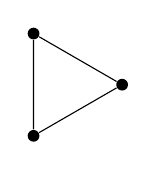
\begin{tikzpicture}[scale=0.3]
\node[v] (A1) at (0:2.5){};
\node[v] (A2) at (120:2.5){};
\node[v] (A3) at (240:2.5){};
\draw (A1)--(A2)--(A3)--(A1);
\end{tikzpicture}
\qquad
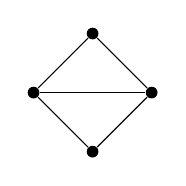
\begin{tikzpicture}[scale=0.3]
\node[v] (A1) at (0:2.5){};
\node[v] (A2) at (90:2.5){};
\node[v] (A3) at (180:2.5){};
\node[v] (A4) at (270:2.5){};

\draw (A1)--(A2)--(A3)--(A4)--(A1);
\draw (A1)--(A3);
\end{tikzpicture}
\qquad
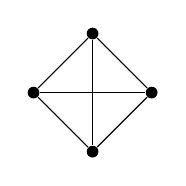
\begin{tikzpicture}[scale=0.3]
\node[v] (A1) at (0:2.5){};
\node[v] (A2) at (90:2.5){};
\node[v] (A3) at (180:2.5){};
\node[v] (A4) at (270:2.5){};

\draw (A1)--(A2)--(A3)--(A4)--(A1);
\draw (A1)--(A3) (A2)--(A4);
\end{tikzpicture}
\qquad
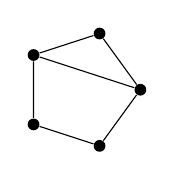
\begin{tikzpicture}[scale=0.3]
\node[v] (A1) at (0:2.5){};
\node[v] (A2) at (72:2.5){};
\node[v] (A3) at (144:2.5){};
\node[v] (A4) at (216:2.5){};
\node[v] (A5) at (288:2.5){};


\draw (A1)--(A2)--(A3)--(A4)--(A5)--(A1);
\draw (A1)--(A3);
\end{tikzpicture}
\qquad
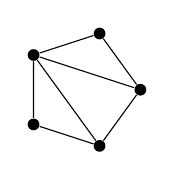
\begin{tikzpicture}[scale=0.3]
\node[v] (A1) at (0:2.5){};
\node[v] (A2) at (72:2.5){};
\node[v] (A3) at (144:2.5){};
\node[v] (A4) at (216:2.5){};
\node[v] (A5) at (288:2.5){};


\draw (A1)--(A2)--(A3)--(A4)--(A5)--(A1);
\draw (A1)--(A3)--(A5);
\end{tikzpicture}
\end{center}
\begin{center}
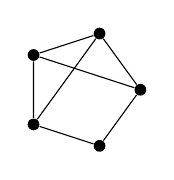
\begin{tikzpicture}[scale=0.3]
\node[v] (A1) at (0:2.5){};
\node[v] (A2) at (72:2.5){};
\node[v] (A3) at (144:2.5){};
\node[v] (A4) at (216:2.5){};
\node[v] (A5) at (288:2.5){};


\draw (A1)--(A2)--(A3)--(A4)--(A5)--(A1);
\draw (A1)--(A3) (A2)--(A4);
\end{tikzpicture}
\qquad
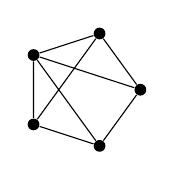
\begin{tikzpicture}[scale=0.3]
\node[v] (A1) at (0:2.5){};
\node[v] (A2) at (72:2.5){};
\node[v] (A3) at (144:2.5){};
\node[v] (A4) at (216:2.5){};
\node[v] (A5) at (288:2.5){};


\draw (A1)--(A2)--(A3)--(A4)--(A5)--(A1);
\draw (A1)--(A3)--(A5) (A2)--(A4);

\end{tikzpicture}
\qquad
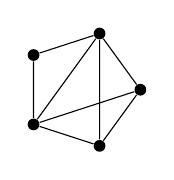
\begin{tikzpicture}[scale=0.3]
\node[v] (A1) at (0:2.5){};
\node[v] (A2) at (72:2.5){};
\node[v] (A3) at (144:2.5){};
\node[v] (A4) at (216:2.5){};
\node[v] (A5) at (288:2.5){};


\draw (A1)--(A2)--(A3)--(A4)--(A5)--(A1);
\draw (A1)--(A4) (A2)--(A5) (A2)--(A4);

\end{tikzpicture}
\qquad
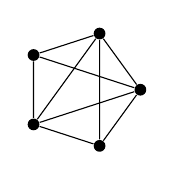
\begin{tikzpicture}[scale=0.3]
\node[v] (A1) at (0:2.5){};
\node[v] (A2) at (72:2.5){};
\node[v] (A3) at (144:2.5){};
\node[v] (A4) at (216:2.5){};
\node[v] (A5) at (288:2.5){};


\draw (A1)--(A2)--(A3)--(A4)--(A5)--(A1);
\draw (A1)--(A3) (A2)--(A5) (A2)--(A4) (A1)--(A4);

\end{tikzpicture}
\qquad
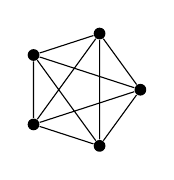
\begin{tikzpicture}[scale=0.3]
\node[v] (A1) at (0:2.5){};
\node[v] (A2) at (72:2.5){};
\node[v] (A3) at (144:2.5){};
\node[v] (A4) at (216:2.5){};
\node[v] (A5) at (288:2.5){};


\draw (A1)--(A2)--(A3)--(A4)--(A5)--(A1);
\draw (A1)--(A3) (A2)--(A4) (A3)--(A5) (A4)--(A1) (A5)--(A2);

\end{tikzpicture}
\end{center}
\glabel{IX}
\end{solution}
\end{enumerate}


\end{document}